\documentclass[11pt,class=report,crop=false]{standalone}
\usepackage[screen]{../python}



\begin{document}

% Commande spécifique
\newcommand{\badletter}[1]{\underline{\textcolor{red}{#1}}}



%====================================================================
\chapitre{Statistique -- Visualisation de données}
%====================================================================

\objectifs{C'est bien de savoir calculer le minimum, le maximum, la moyenne, les quartiles d'une série. C'est encore mieux de les visualiser tous sur un même graphique !}


%%%%%%%%%%%%%%%%%%%%%%%%%%%%%%%%%%%%%%%%%%%%%%%%%%%%%%%%%%%%%%%%
% Activité 1
%%%%%%%%%%%%%%%%%%%%%%%%%%%%%%%%%%%%%%%%%%%%%%%%%%%%%%%%%%%%%%%%

\begin{activite}[Statistique de base]

\objectifs{Objectifs : calculer les principales caractéristiques 
d'une série de données : minimum, maximum, moyenne et écart-type.}

Dans cette activité \ci{liste} désigne une liste de nombres (entiers ou flottants). 

\begin{enumerate}
  \item Écris ta propre fonction \ci{somme(liste)} qui calcule la somme des éléments d'une liste donnée.
  Compare ton résultat avec la fonction \ci{sum()} décrite ci-dessous qui existe déjà en \Python{}. En particulier pour une liste vide vérifie que ton résultat est bien $0$. 
  
  \index{sum@\ci{sum}}
  
  \begin{fonctionpython}[\ci{python : sum()}]
   Usage : \ci{sum(liste)}\\
   Entrée : une liste de nombres\\
   Sortie : un nombre
  
  \medskip
     
   Exemple : \ci{sum([4,8,3])} renvoie \ci{15}
  \end{fonctionpython}   
  
  \emph{Tu peux maintenant utiliser la fonction \ci{sum()} dans tes programmes !}
  
  
  \item Écris une fonction \ci{moyenne(liste)} qui calcule la moyenne des éléments d'une liste donnée (et renvoie $0$ si la liste est vide).\index{moyenne}
  
  \item Écris ta propre fonction \ci{minimum(liste)} qui renvoie la plus petite valeur des éléments d'une liste donnée. Compare ton résultat avec la fonction \Python{} \ci{min()} décrite ci-dessous (qui en plus sait calculer le minimum de deux nombres).
  
  \index{min@\ci{min}}  
  
  \begin{fonctionpython}[\ci{python : min()}]
   Usage : \ci{min(liste)} \  ou \  \ci{min(a,b)}\\
   Entrée : une liste de nombres ou bien deux nombres\\
   Sortie : un nombre
  
  \medskip
     
   Exemple : 
  \begin{itemize}  
    \item \ci{min(12,7)} renvoie \ci{7}  
    \item \ci{min([10,5,9,12])} renvoie \ci{5}
  \end{itemize}    

  \end{fonctionpython}   
  
  \emph{Tu peux maintenant utiliser la fonction \ci{min()}, et aussi bien sûr la fonction \ci{max()} dans tes programmes !}\index{max@\ci{max}} 
  
  \item La \defi{variance}\index{variance} d'une série de données $(x_1,x_2,\ldots,x_n)$ est définie comme la moyenne des carrés des écarts à la moyenne. C'est-à-dire :
  $$v = \frac{1}{n}\big((x_1-m)^2 + (x_2-m)^2 + \cdots + (x_n-m)^2\big)$$
  où $m$ est la moyenne de $(x_1,x_2,\ldots,x_n)$.
  
  Écris une fonction \ci{variance(liste)} qui calcule la variance des éléments d'une liste.
  
  Par exemple, pour la série $(6,8,2,10)$, la moyenne est $m = 8$, la variance est
  $$v = \frac{1}{4} = \big((6-8)^2 + (8-8)^2 + (2-8)^2 + (10-8)^2\big) = 8.75.$$
  
  \item L'\defi{écart-type}\index{ecart-type@écart-type} d'une série $(x_1,x_2,\ldots,x_n)$ est la racine carrée de la variance :
  $$e = \sqrt{v}$$
  où $v$ est la variance. Programme une fonction \ci{ecart_type(liste)}.
  
%  La fonction racine carrée \ci{sqrt()} n'est pas disponible par défaut dans \Python. Pour l'utiliser, il faut appeler le module des fonctions mathématiques par la commande :\\
%  \centerline{\ci{from math import *}}

  \item Voici les températures mensuelles moyennes à Brest et à Strasbourg.
  \centerline{\ci{temp_brest = [6.4,6.5,8.5,9.7,11.9,14.6,15.9,16.3,15.1,12.2,9.2,7.1]}}
  \centerline{\ci{temp_strasbourg = [0.9,2.4,6.1,9.7,13.8,17.2,19.2,18.6,15.7,10.7,5.3,2.1]}}

  Calcule la température moyenne sur l'année à Brest puis à Strasbourg. Calcule l'écart-type 
  des températures à Brest puis à Strasbourg. Quelles conclusions en tires-tu ? 

\end{enumerate}

\end{activite}



%%%%%%%%%%%%%%%%%%%%%%%%%%%%%%%%%%%%%%%%%%%%%%%%%%%%%%%%%%%%%%%%
%%%%%%%%%%%%%%%%%%%%%%%%%%%%%%%%%%%%%%%%%%%%%%%%%%%%%%%%%%%%%%%%

\begin{cours}[Graphiques avec tkinter]

\index{tkinter@\ci{tkinter}}
\index{module!tkinter@\ci{tkinter}}
\index{graphique}
\index{fenetre@fenêtre}

Pour afficher ceci :
\begin{center}
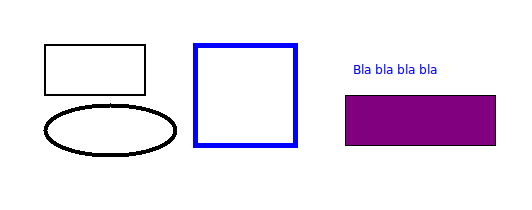
\includegraphics[scale=0.6]{ecran-stat-cours-intro}
\end{center}
Le code est :
\begin{lstlisting}
# Module tkinter
from tkinter import *

# Fenêtre tkinter
root = Tk()
        
canvas = Canvas(root, width=800, height=600, background="white")
canvas.pack(fill="both", expand=True)

# Un rectangle
canvas.create_rectangle(50,50,150,100,width=2)

# Un rectangle à gros bords bleus
canvas.create_rectangle(200,50,300,150,width=5,outline="blue")

# Un rectangle rempli de violet
canvas.create_rectangle(350,100,500,150,fill="purple")

# Un ovale
canvas.create_oval(50,110,180,160,width=4)

# Du texte
canvas.create_text(400,75,text="Bla bla bla bla",fill="blue")

# Ouverture de la fenêtre
root.mainloop()
\end{lstlisting}


Quelques explications :
\begin{itemize}
  \item Le module \ci{tkinter} nous permet de définir des variables \ci{root} et \ci{canvas} qui définissent une fenêtre graphique (ici de largeur $800$ et de hauteur $600$ pixels).
  On décrit ensuite tout ce que l'on veut ajouter dans la fenêtre. Et enfin la fenêtre est affichée par la commande \ci{root.mainloop()} (tout à la fin). 
  
    
  \item Attention ! Le repère graphique de la fenêtre a son axe des ordonnées dirigé vers le bas. L'origine $(0,0)$ est le coin en haut à gauche (voir la figure ci-dessous). 
  
  \item Commande pour tracer un rectangle : \ci{create_rectangle(x1,y1,x2,y2)} ; il suffit de préciser les coordonnées $(x_1,y_1)$, $(x_2,y_2)$ de deux sommets opposés. L'option \ci{width} ajuste l'épaisseur du trait, \ci{outline} définit la couleur de ce trait, \ci{fill} définit la couleur de remplissage.
  
  \item Une ellipse est tracée par la commande \ci{create_oval(x1,y1,x2,y2)}, où $(x_1,y_1)$, $(x_2,y_2)$ sont les coordonnées de deux sommets opposés d'un rectangle encadrant l'ellipse voulue (voir la figure). On obtient un cercle lorsque le rectangle correspondant est un carré !  
  
  \item Du texte est affiché par la commande \ci{canvas.create_text(x,y,text="Mon texte")} en précisant les coordonnées $(x,y)$ du point à partir duquel on souhaite afficher le texte. 
  
\end{itemize}

\myfigure{0.8}{
\tikzinput{fig-stat-cours-intro}
}

\end{cours}


%%%%%%%%%%%%%%%%%%%%%%%%%%%%%%%%%%%%%%%%%%%%%%%%%%%%%%%%%%%%%%%%
% Activité 2
%%%%%%%%%%%%%%%%%%%%%%%%%%%%%%%%%%%%%%%%%%%%%%%%%%%%%%%%%%%%%%%%

\begin{activite}[Graphiques]

\objectifs{Objectifs : visualiser des données par différents types de graphiques.}

\begin{center}
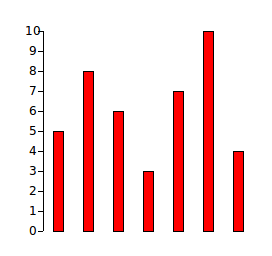
\includegraphics[width=5cm]{ecran-stat-2a}\qquad\qquad
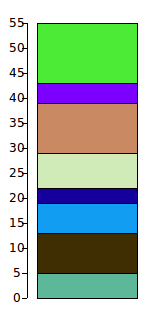
\includegraphics[height=5cm]{ecran-stat-2b}

\qquad\qquad\textbf{Graphique en barres}\qquad\qquad\quad
\textbf{Graphique cumulatif}
\end{center}

\begin{center}
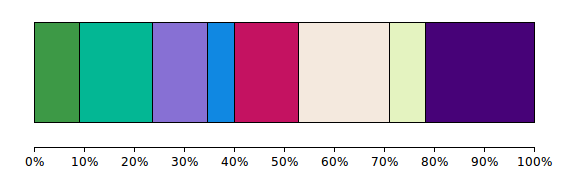
\includegraphics[width=7cm]{ecran-stat-2c}\qquad\qquad
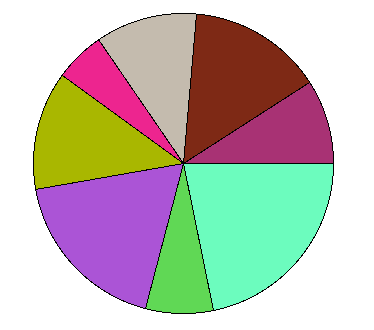
\includegraphics[width=4cm]{ecran-stat-2d}

\qquad\qquad\textbf{Graphique en pourcentage}\qquad\qquad\qquad
\textbf{Graphique en secteurs}
\end{center}

\begin{enumerate}
  \item \textbf{Graphique en barres.} Écris une fonction \ci{graphique_barres(liste)} qui affiche les valeurs d'une liste sous la forme de barres verticales.
  


 Indications :
  \begin{itemize}
    \item Dans un premier temps, ne t'occupe pas de tracer l'axe vertical des coordonnées avec les indications chiffrées.
    \item Tu peux définir une variable \ci{echelle} qui permet d'agrandir tes rectangles, afin qu'ils aient une taille adaptée à l'écran.
    \item Si tu souhaites tester ton graphique avec une liste au hasard voici comment construire une liste aléatoire de $10$ entiers compris entre $1$ et $20$ :
    
\begin{lstlisting}
from random import *
liste = [randint(1,20) for i in range(10)]
\end{lstlisting}

\end{itemize}

  \item \textbf{Graphique cumulatif.} Écris une fonction \ci{graphique_cumulatif(liste)} qui affiche les valeurs d'une liste sous la forme de rectangles les uns au-dessus des autres.
  

  
  \item \textbf{Graphique en pourcentage.} Écris une fonction \ci{graphique_pourcentage(liste)} qui affiche les valeurs d'une liste sous la forme d'un rectangle horizontal de taille fixe (par exemple $500$ pixels) et qui est divisé en sous-rectangles représentant les valeurs.
  


  \item \textbf{Graphique en secteurs.} Écris une fonction \ci{graphique_secteurs(liste)} qui affiche les valeurs d'une liste sous la forme d'un disque de taille fixe et divisé en secteurs représentant les valeurs. 
 
La fonction \ci{create_arc()}, qui permet de dessiner des arcs de cercles, n'est pas très intuitive. Il faut penser que l'on dessine un cercle, en précisant les coordonnées des coins d'un carré qui l'entoure, puis en précisant l'angle de début et l'angle du secteur (en degrés). 


\centerline{\ci{canvas.create_arc(x1,y1,x2,y2,start=debut_angle,extent=mon_angle)}}


\myfigure{1}{
\tikzinput{fig-stat-arc}
}
L'option \ci{style=PIESLICE} affiche un secteur au lieu d'un arc. 


  \item \textbf{Bonus.} Rassemble ton travail en un programme qui laisse la possibilité à l'utilisateur de choisir le diagramme qu'il souhaite en cliquant sur des boutons, et aussi la possibilité d'obtenir une nouvelle série aléatoire de données. \emph{Pour afficher et gérer les boutons avec \ci{tkinter}, vois le cours ci-dessous.}
  
\begin{center}
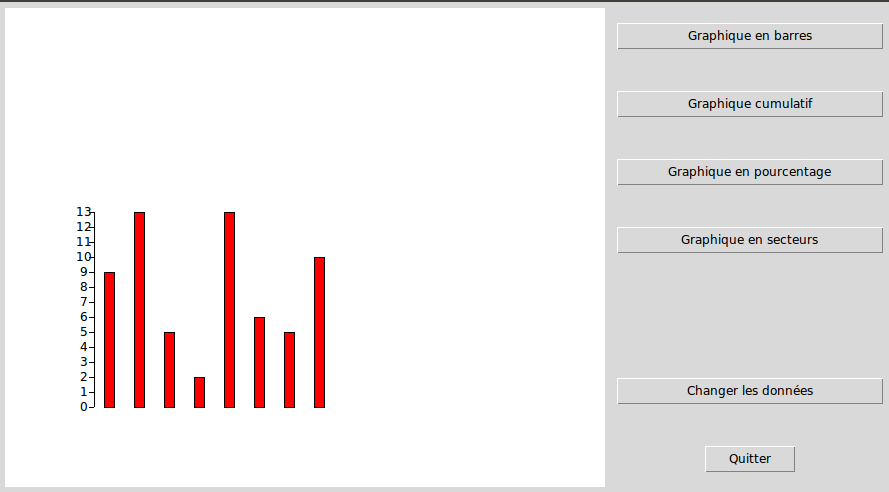
\includegraphics[scale=0.4]{ecran-stat-2e}
\end{center}   
  \end{enumerate}
\end{activite}


%%%%%%%%%%%%%%%%%%%%%%%%%%%%%%%%%%%%%%%%%%%%%%%%%%%%%%%%%%%%%%%%
%%%%%%%%%%%%%%%%%%%%%%%%%%%%%%%%%%%%%%%%%%%%%%%%%%%%%%%%%%%%%%%%

\begin{cours}[Boutons avec tkinter]

\index{bouton}

Il est plus ergonomique d'afficher des fenêtres où les actions sont exécutées en cliquant sur des boutons.

Voici la fenêtre d'un petit programme avec deux boutons. Le premier bouton change la couleur du rectangle, le second termine le programme.
\begin{center}
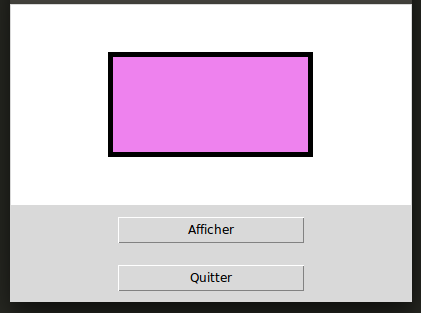
\includegraphics[scale=0.6]{ecran-stat-cours-boutons}
\end{center}
Le code est :
\begin{lstlisting}
from tkinter import *
from random import *

root = Tk()     
canvas = Canvas(root, width=400, height=200, background="white")
canvas.pack(fill="both", expand=True)

def action_bouton():
    canvas.delete("all")         # Efface tout
    couleurs = ["red","orange","yellow","green","cyan","blue","violet","purple"]
    coul = choice(couleurs)      # Couleur au hasard
    canvas.create_rectangle(100,50,300,150,width=5,fill=coul)
    return

bouton_couleur = Button(root,text="Afficher", width=20, command=action_bouton)
bouton_couleur.pack()

bouton_quitter = Button(root,text="Quitter", width=20, command=root.quit)
bouton_quitter.pack()

root.mainloop()
\end{lstlisting}

Quelques explications :
\begin{itemize}
  \item On crée un bouton par la commande \ci{Button}. L'option \ci{text} personnalise le texte qui s'affiche sur le bouton. On ajoute le bouton créé à la fenêtre par la méthode \ci{pack}.
  \item Le plus important est l'action associée au bouton ! C'est l'option \ci{command} qui reçoit le nom de la fonction à exécuter lorsque le bouton est cliqué. Pour notre exemple \ci{command=action_bouton}, associe au clic sur le bouton un changement de couleur.
  
  \item Attention ! il faut donner le nom de la fonction sans parenthèses : \ci{commande=ma_fonction} et pas \ci{command=ma_fonction()}.
  
  \item Pour associer au bouton \og{}Quitter\fg{} la fermeture du programme, l'argument est \ci{command=root.quit}.
  
  \item La commande \ci{canvas.delete("all")} efface tous les dessins de notre fenêtre graphique.
  
\end{itemize}
\end{cours}


%%%%%%%%%%%%%%%%%%%%%%%%%%%%%%%%%%%%%%%%%%%%%%%%%%%%%%%%%%%%%%%%
% Activité 3
%%%%%%%%%%%%%%%%%%%%%%%%%%%%%%%%%%%%%%%%%%%%%%%%%%%%%%%%%%%%%%%%

\begin{activite}[Médiane et quartiles]

\objectifs{Objectifs : calculer la médiane et les quartiles d'un effectif.}



%\begin{center}
%\includegraphics[scale=1]{}
%\end{center}

\begin{enumerate}
  \item Écris une fonction \ci{mediane(liste)}\index{mediane@médiane} qui calcule la valeur médiane des éléments d'une liste donnée. Par définition, la moitié des valeurs est inférieure ou égale à la médiane, l'autre moitié est supérieure ou égale à la médiane.

  \emph{Rappels.} On note $n$ la longueur de la liste et on suppose que la liste est ordonnée (du plus petit au plus grand élément).
  \begin{itemize}
    \item \textbf{Cas $n$ impair.} La médiane est la valeur de la liste au rang $\frac{n-1}{2}$.    
    Exemple avec \ci{liste = [12,12,14,15,19]} :
    \begin{itemize}
      \item la longueur de la liste est $n=5$ (les indices vont de $0$ à $4$),
      \item l'indice du milieu est l'indice $2$,
      \item la médiane est la valeur \ci{liste[2]}, c'est donc $14$.
    \end{itemize}
    
    \item \textbf{Cas $n$ pair.} La médiane est la moyenne entre la valeur de la liste au rang $\frac{n}{2}-1$ et au rang $\frac{n}{2}$.
    Exemple avec \ci{liste = [13,14,19,20]} :
    \begin{itemize}
      \item la longueur de la liste est $n=4$ (les indices vont de $0$ à $3$),
      \item les indices du milieu sont $1$ et $2$,
      \item la médiane est la moyenne entre \ci{liste[1]} et \ci{liste[2]}, c'est donc $\frac{14+19}{2} = 16.5$.
    \end{itemize}    
   \end{itemize} 
   
   
   
     
    \item Les résultats d'une classe sont collectés sous la forme suivante d'un effectif par note : \\
    \centerline{\ci{effectif_notes = [0,0,0,0,0,1,0,2,0,1,5,1,2,3,2,4,1,2,0,1,0]}} 
    Le rang $i$ va de $0$ à $20$. Et la valeur au rang $i$ indique le nombre d'élèves ayant eu la note $i$.
    Par exemple ici, $1$ élève a eu la note $5$, $2$ élèves ont eu la note $7$,\ldots , $5$ élèves ont obtenus $10$, \ldots{}  
    Écris une fonction \ci{notes_vers_liste(effectif_notes)} qui prend en entrée un effectif de notes et renvoie la liste des notes. Pour notre exemple la fonction doit renvoyer \ci{[5,7,7,9,10,10,10,10,10,10,...]}.
       
    Déduis-en une fonction qui calcule la médiane des notes d'une classe à partir d'un effectif par note.
    
    \item Écris une fonction \ci{calcule_quartiles(liste)} qui calcule les quartiles $Q_1$, $Q_2$, $Q_3$ des éléments d'une liste donnée. Les quartiles\index{quartiles} répartissent les valeurs en : un quart en-dessous de $Q_1$, un quart entre $Q_1$ et $Q_2$, un quart entre $Q_2$ et $Q_3$, un quart au-dessus de $Q_3$.
    Pour le calcul, on utilisera que :
    \begin{itemize}
      \item $Q_2$ est simplement la médiane de la liste entière (supposée ordonnée),
      \item $Q_1$ est la médiane de la sous-liste formée de la première moitié des valeurs,
      \item $Q_3$ est la médiane de la sous-liste formée de la seconde moitié des valeurs. 
    \end{itemize}           
\end{enumerate}

  Pour l'implémentation, il faut une nouvelle fois discuter selon que la longueur $n$ de la liste est paire ou pas.
  
  Déduis-en une fonction qui calcule les quartiles des notes d'une classe à partir d'un effectif par note.

\end{activite}


%%%%%%%%%%%%%%%%%%%%%%%%%%%%%%%%%%%%%%%%%%%%%%%%%%%%%%%%%%%%%%%%
% Activité 4
%%%%%%%%%%%%%%%%%%%%%%%%%%%%%%%%%%%%%%%%%%%%%%%%%%%%%%%%%%%%%%%%

\begin{activite}[Diagramme en boîte]

\objectifs{Objectifs : tracer des diagrammes en boîte.}

Un \defi{diagramme en boîte} (appelé aussi \defi{boîte à moustaches}) est un graphique qui représente les principales caractéristiques d'une série statistique : minimum, maximum, médiane et quartiles. Le schéma de principe est le suivant :

\myfigure{0.45}{
  \tikzinput{fig-stat-boite}
} 

Écris une fonction \ci{diagramme_boite(effectif_notes)} qui trace le diagramme en boîte des notes d'une classe à partir d'un effectif par note (voir l'activité précédente).

\begin{center}
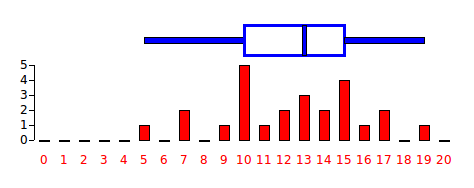
\includegraphics[scale=0.7]{ecran-stat-4}
\end{center}

\end{activite}



%%%%%%%%%%%%%%%%%%%%%%%%%%%%%%%%%%%%%%%%%%%%%%%%%%%%%%%%%%%%%%%%
% Activité 5
%%%%%%%%%%%%%%%%%%%%%%%%%%%%%%%%%%%%%%%%%%%%%%%%%%%%%%%%%%%%%%%%

\begin{activite}[Moyenne mobile]

\objectifs{Objectifs : calculer des moyennes mobiles afin de \og{}lisser\fg{} des courbes.}

\index{moyenne}

\begin{enumerate}
  \item Simule le cours de la bourse de l'indice \emph{Top 40} sur 365 jours.
  Au jour $j=0$, l'indice vaut $1000$. Ensuite l'indice d'un jour est déterminé en ajoutant une valeur au hasard (positive ou négative) à la valeur de l'indice de la veille :\\
  \centerline{indice du jour $j$ = indice du jour $(j-1)$ \ + \ valeur au hasard}.
  
  Pour cette valeur au hasard, tu peux essayer une formule du style :\\
  \centerline{\ci{valeur = randint(-10,12)/3}}
  
  Écris une fonction \ci{cours_bourse()}, sans paramètre, qui renvoie une liste de $365$ valeurs de l'indice \emph{Top 40} selon cette méthode.
  
  \item Trace point par point la courbe du cours sur une année. (Pour tracer un point, tu peux afficher un carré de taille $1$ pixel.)
  
\begin{center}
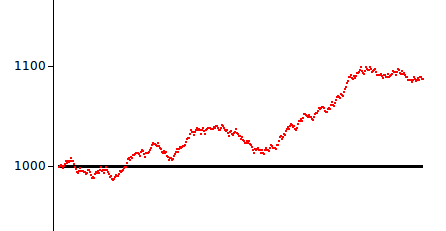
\includegraphics[scale=0.7]{ecran-stat-5a}
\end{center}

   \item \emph{Comme la courbe du cours journalier est très chaotique, nous souhaitons la lisser afin de la rendre plus lisible. Pour cela nous calculons des moyennes mobiles.}
   
   La moyenne mobile à $7$ jours pour le jour $j$, est la moyenne des $7$ derniers cours. Par exemple : la moyenne mobile (à $7$ jours) pour le jour $j = 7$ est la moyenne des cours des jours $j=1,2,3,4,5,6,7$. On peut changer la durée : par exemple la moyenne mobile à $30$ jours est la moyenne des $30$ derniers cours.
   
   Écris une fonction \ci{moyenne_mobile(liste,duree)} qui renvoie la liste de toutes les moyennes mobiles d'une série de données, pour une durée fixée.
   
    \item Trace point par point sur un même graphique : la courbe du cours sur une année (en rouge ci-dessous), la courbe de ses moyennes mobiles à $7$ jours (en bleu ci-dessous) et la courbe des ses moyennes mobiles à $30$ jours (en marron ci-dessous). Note que plus la durée est longue plus la courbe est \og{}lisse\fg{}. (Bien sûr la courbe des moyennes mobiles à $30$ jours ne commence qu'à partir du trentième jour.)
   
\begin{center}
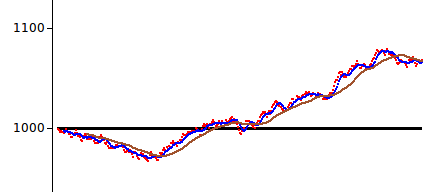
\includegraphics[scale=0.7]{ecran-stat-5b}
\end{center}

\end{enumerate}

\end{activite}


\end{document}
